\clearpage
\item \subquestionpoints{5} \textbf{Coding problem.}
We now consider the case where the $t$-labels are unavailable, so you only have
access to the $y$-labels at training time. Add to your code in
\texttt{p02cde\_posonly.py} to re-train the classifier (still using $x_1$ and
$x_2$ as input features), but using the $y$-labels only.

\ifnum\solutions=1 {
  \begin{answer}
\newline
  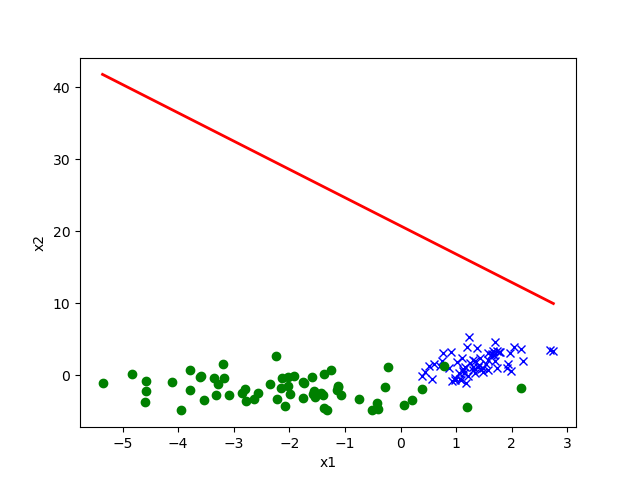
\includegraphics[height=10cm]{C:/Users/feroc/OneDrive/Notability/CS229 Machine Learning/problem_sets/ps1/src/output/p02d_pred.png}
\end{answer}

} \fi
